\documentclass[a4paper, fleqn]{article}
\usepackage[utf8]{inputenc}
\usepackage{amsmath}
\usepackage{amssymb}
\usepackage{caption}
\usepackage{mathtools}
\usepackage{amsfonts}
\usepackage{lastpage}
\usepackage{tikz}
\usepackage{float}
\usepackage{textcomp}
\usepackage{kbordermatrix}
\usetikzlibrary{patterns}
\usepackage{pdfpages}
\usepackage{gauss}
\usepackage{fancyvrb}
\usepackage[table]{colortbl}
\usepackage{fancyhdr}
\usepackage{graphicx}
\usepackage[margin=2.5 cm]{geometry}

\setlength\parindent{0pt}
\setlength\mathindent{75pt}

\definecolor{listinggray}{gray}{0.9}
\usepackage{listings}
\lstset{
	language=,
	literate=
		{æ}{{\ae}}1
		{ø}{{\o}}1
		{å}{{\aa}}1
		{Æ}{{\AE}}1
		{Ø}{{\O}}1
		{Å}{{\AA}}1,
	backgroundcolor=\color{listinggray},
	tabsize=3,
	rulecolor=,
	basicstyle=\scriptsize,
	upquote=true,
	aboveskip={0.2\baselineskip},
	columns=fixed,
	showstringspaces=false,
	extendedchars=true,
	breaklines=true,
	prebreak =\raisebox{0ex}[0ex][0ex]{\ensuremath{\hookleftarrow}},
	frame=single,
	showtabs=false,
	showspaces=false,
	showlines=true,
	showstringspaces=false,
	identifierstyle=\ttfamily,
	keywordstyle=\color[rgb]{0,0,1},
	commentstyle=\color[rgb]{0.133,0.545,0.133},
	stringstyle=\color[rgb]{0.627,0.126,0.941},
  moredelim=**[is][\color{blue}]{@}{@},
}

\lstdefinestyle{base}{
  emptylines=1,
  breaklines=true,
  basicstyle=\ttfamily\color{black},
}

\pagestyle{fancy}
\def\checkmark{\tikz\fill[scale=0.4](0,.35) -- (.25,0) -- (1,.7) -- (.25,.15) -- cycle;}
\newcommand*\circled[1]{\tikz[baseline=(char.base)]{
            \node[shape=circle,draw,inner sep=2pt] (char) {#1};}}
\newcommand*\squared[1]{%
  \tikz[baseline=(R.base)]\node[draw,rectangle,inner sep=0.5pt](R) {#1};\!}
\newcommand{\comment}[1]{%
  \text{\phantom{(#1)}} \tag{#1}}
\def\el{[\![}
\def\er{]\!]}
\def\dpip{|\!|}
\def\MeanN{\frac{1}{N}\sum^N_{n=1}}
\cfoot{Page \thepage\ of \pageref{LastPage}}
\DeclareGraphicsExtensions{.pdf,.png,.jpg}
\author{Nikolaj Dybdahl Rathcke (Student ID: 74763954)}
\title{Combinatorics \\ Assignment 1}
\lhead{Combinatorics}
\rhead{Assignment 1}

\begin{document}
\maketitle

\section*{Question 1}
TODO

\section*{Question 3}
To do this, we need to show that (a) implies (b), that (b) implies (c) and that (c) implies (a).\\
(a) $\Rightarrow$ (b): If $e$ is a loop, then any subset containing $e$ must be dependent and therefore cannot be a basis. \\
(b) $\Rightarrow$ (c): If $e$ is no bases, then by $(I2)$, it cannot be in any independent sets, as all independent sets in $\mathcal{I}$ are subsets of the bases. \\
(c) $\Rightarrow$ (a): If $e$ is in no independent sets, then it must be a loop, as otherwise the set $\{e\}$ would be an independent set.

\section*{Question 4}
TODO

\section*{Question 5}
TODO

\section*{Question 6}
TODO

\section*{Question 7}
TODO

\section*{Question 8}
We solve this using Prim's algorithm. We start by picking a vertex, say $a$, and then pick the edge with the lowest weight. We keep picking an edge with minimum weight that is adjacent to the tree we are creating, and that includes a vertex that is not currently in the tree. The algorithm runs as follows (use Figure \ref{fig1} for reference:
\begin{enumerate}
  \item Both edges adjacent to $a$ have weight $6$, so it does not matter what we pick. So we pick $(a,b)$.
  \item The edge $(b,e)$ has the lowest weight, so we pick that one.
  \item The edge $(e,f)$ now has the lowest weight, so we pick that one.
  \item We can either pick $(e,g)$ or $(f,g)$ as they both have weight $3$. In this case we pick $(e,g)$.
  \item The edge with lowest weight which includes a vertex not currently in the tree is $(e,c)$.
  \item Finally, we pick the edge $(c,d)$ and we have a minimum spanning tree.
\end{enumerate}
This minimum spanning tree is not unique as we could have picked $(a,g)$ instead of $(a,b)$ as well as $(f,g)$ instead of $(e,g)$.
\begin{figure}[H]
  \centering
  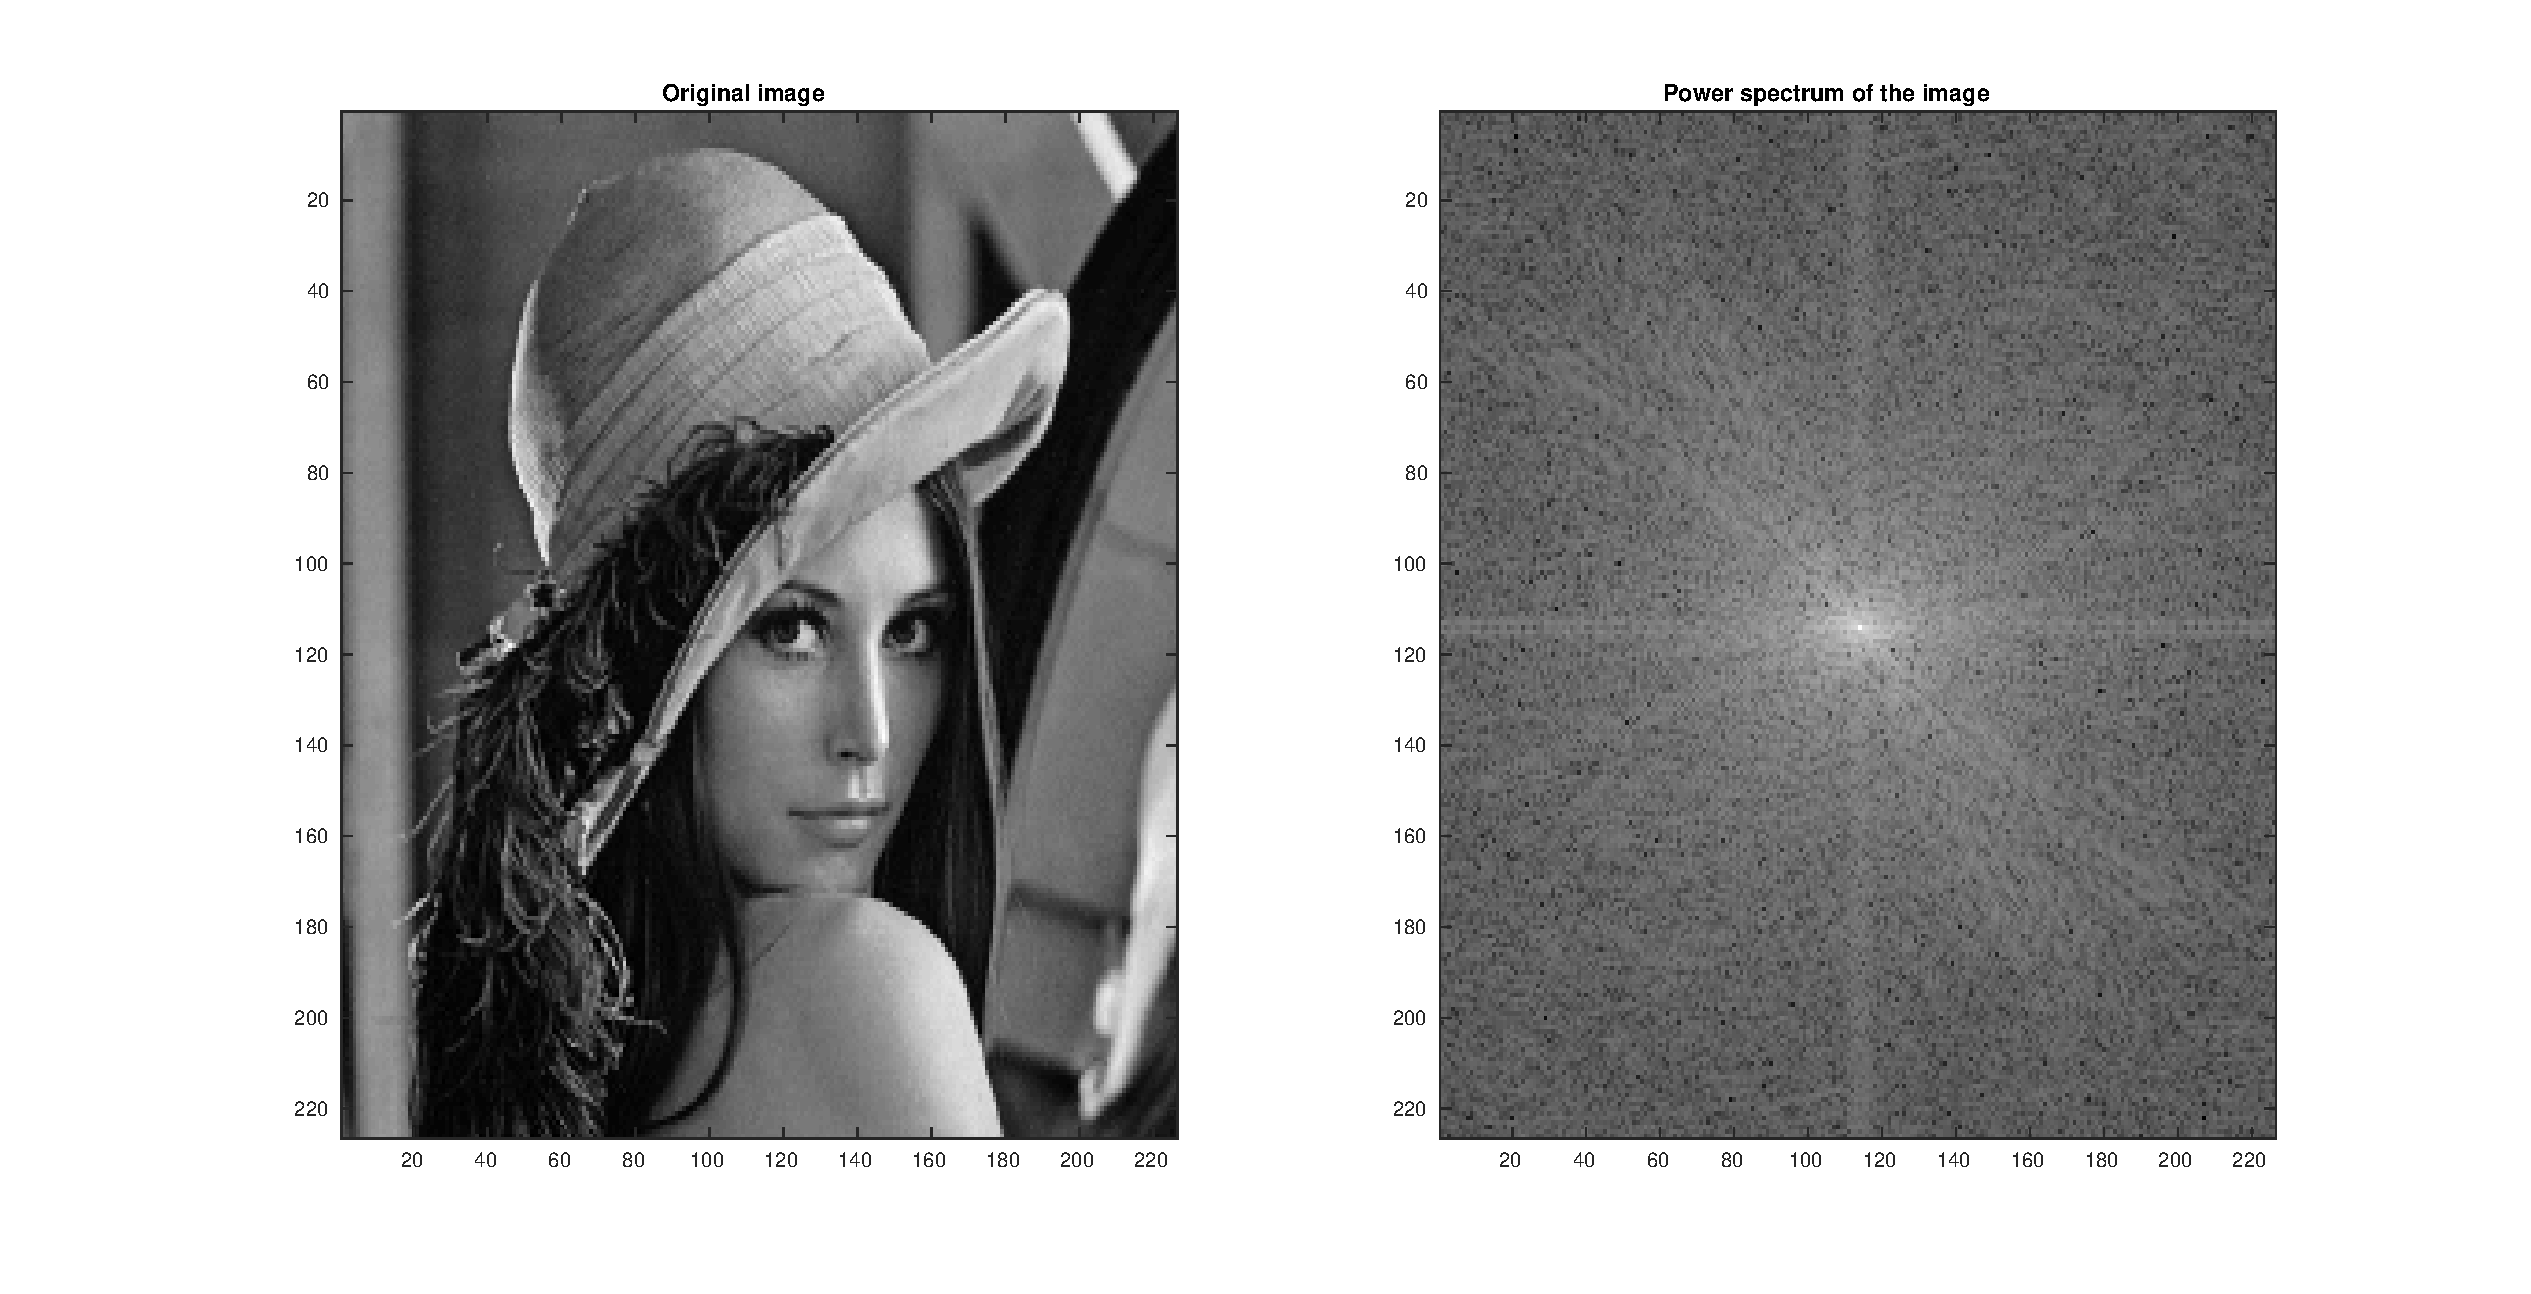
\includegraphics[scale=0.6]{fig1}
  \caption{A minimum spanning tree produced by Prim's Algorithm}
  \label{fig1}
\end{figure}

\section*{Question 9}
TODO

\section*{Question 11}
TODO







\end{document}
